% !TEX root = Main.tex

\section{Vorgehen während der Entwicklung und Implementierung der Sprache}
Dieser Abschnitt beschreibt unser Vorgehen während der Entwicklung der Programmiersprache. Ein Unterabschnitt stellt dabei jeweils einen Entwicklungsschritt des Compilers da. Um diese Abschnitte besser verständlich zu machen, wird teilweise von Kapitel \ref{sec:verwendung}. \textit{Verwendung der UnsereCompilerbauSprache} vorgegriffen.
\subsection{Erste Schritte: Auswertung von arithmetischen Ausdrücken}
\label{subsec:arithExp}
Der Vorgehensweise unter \textit{\ref{sec:grundsatz}. Allgemeiner Grundsatz} entsprechend, implementierten wir zuerst die unserer Sicht nach grundlegendste Fähigkeit einer Programmiersprache: das Auswerten von arithmetischen Ausdrücken. Es soll möglich sein, Ausdrücke, die die Grundrechenarten sowie eine beliebig tiefe Schachtelung von Klammern enthalten, zu erkennen und der Operatorenpriorität entsprechend die gelesenen Tokens in einem Syntaxbaum zusammenzuführen. Dazu formulierten wir folgende Grammatik:


\scriptsize\begin{lstlisting} [frame=single] 
//Datei: Arithmetic.g4
grammar Arithmetic;

///////////////////////////////////////////////////////
// beliebige Folge der Ziffern 0 bis 9
INTEGER : [0-9]+ ;        
// ueberspringt Leerzeichen, Tabstops sowie Linefeeds
WS : [ \t\r\n]+ -> skip ; 
// oeffndende runde Klammer
LPAREN : '(';		  	  
// schliessende runde Klammer
RPAREN : ')';		  	  
///////////////////////////////////////////////////////
//mathematische Operatoren
PLUSOP : '+';
MINOP : '-';
MULTOP : '*';
DIVOP : '/';
///////////////////////////////////////////////////////
//Regeln fuer math. Ausdruecke
expression: INTEGER					
	| LPAREN expression RPAREN		
	| expression DIVOP  expression  
	| expression MULTOP expression	
	| expression MINOP  expression 
	| expression PLUSOP expression 
	;			
///////////////////////////////////////////////////////

\end{lstlisting}
\normalsize
Eine Grammatik für ANTLR hat folgenden Aufbau:

Die Definition der Grammatik beginnt mit dem Schlüsselwort ''grammar'' sowie dem Namen der Grammatik. Dabei gilt es zu beachten, dass die Datei den gleichen Namen wie die Grammatik selbst sowie die Dateiendung ''.g4'' besitzt. Diese Deklaration wird mit einem Semikolon abgeschlossen.

Zeilen, die mit ''//'' beginnen, sind Kommentare und haben keinen Einfluss auf die Grammatik. Sie dienen lediglich als Erläuterungen und zur Formatierung, um die Lesbarkeit zu verbessern.

Auf die Deklaration dürfen beliebig viele Regeln für die Grammatik folgen. Zur Formulierung der Regeln werden reguläre Ausdrücke genutzt. Beispielsweise besagt die sechste Zeile, dass es eine Regel INTEGER gibt, wobei ein INTEGER sich aus einer beliebigen Folge der Ziffern von 0 bis 9 zusammensetzt. Der reguläre Ausdruck [0-9] gibt an, dass ein beliebiges Zeichen im Bereich von 0 bis 9 vorkommen darf. Das abschließende ''+'' bedeutet, dass es sich um eine Kette dieser Zeichen, die beliebig lange ist, jedoch mindestens die Länge 1 besitzt, handelt.

Die Regel WS (Whitespace) besagt, dass bestimmte Zeichen, die nur der Formatierung dienen, ignoriert werden, da sie für das Übersetzen einer Quelldatei keine Bedeutung haben.

Die darauffolgenden Regeln sind Aliase für die Zeichen, die in arithmetischen Ausdrücken verwendet werden. Diese Auslagerung steigert unseres Erachtens nach die Lesbarkeit der letzten Regeln dieses Beispiels, sind aber nicht zwingend notwendig.

Die wohl relevanteste Regel trägt den Namen ''expression'' und legt fest, wie sich ein arithmetischer Ausdruck zusammensetzen kann. Im Vergleich zu den vorherigen Regeln, wurde hier von der Möglichkeit, mehrere alternative Möglichkeiten anzugeben, Gebrauch gemacht. Die Regel besagt, dass ein arithmetischer Ausdruck entweder aus 
\begin{itemize}
\item einer Zahl,
\item einem geklammerten Ausdruck,
\item einer Division mit zwei Operanden,
\item einer Multiplikation mit zwei Operanden,
\item einer Subtraktion mit zwei Operanden
\item oder einer Addition mit zwei Operanden
\end{itemize}
besteht.
Durch die Rekursion (die Regel verweist auf sich selbst) ist eine beliebige Länge des Ausdruckes möglich.

Eine Besonderheit, die zu beachten ist, besteht in der Rangfolge der Operatoren. Die höchste Bindung besitzt ein geklammerter Term, die nächst höchste Bindung Divisionen und Multiplikationen. Die schwächste Bindung besitzen Subtraktionen und Additionen.

Damit diese Priorität gewährleistet werden kann, sind die Regeln in dieser bestimmten Reihenfolge notiert. ANTLR versucht immer zuerst die ''oberste'' Regel anzuwenden, daraufhin die darunter stehende usw.. Deshalb wird der folgende Ausdruck 

\begin{lstlisting} [frame=single]
2*10-48*(4-1)-16/4
\end{lstlisting}

zu diesem Syntaxbaum aufgelöst:

\begin{figure}[h!]
\centering
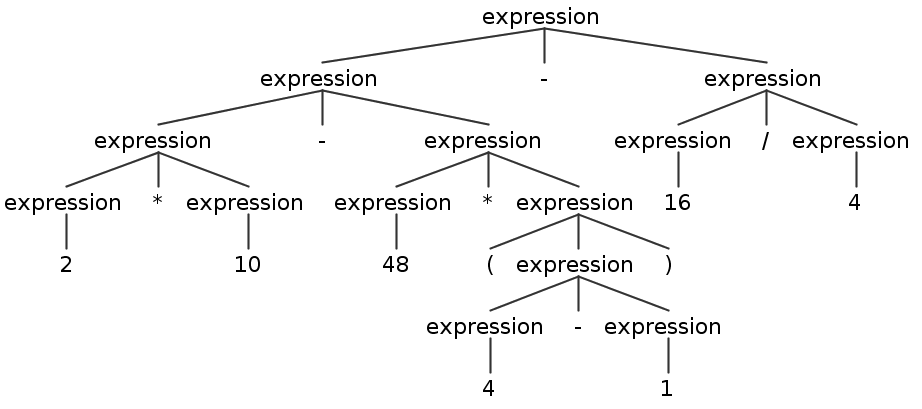
\includegraphics[scale=0.4]{pics/antlr4_parse_tree_arithmetic.png}
\caption{Syntaxbaum für beispielhaften arithmetischen Ausdruck}
\end{figure}

Des Weiteren ist zu beachten, dass arithmetischen Ausdrücke gleicher Operatorenpriorität von links  nach rechts ausgewertet werden müssen. Als Beispiel lässt sich hier der Term 
\begin{lstlisting} [frame=single]
8-5+2
\end{lstlisting}
nennen. Sowohl die Subtraktion als auch die Addition besitzen die gleiche Bindung. Wenn man hier fälschlicherweise zuerst die Addition, also 5+2, was 7 ergibt, auswertet und das Ergebnis dieser Operation von 8 subtrahiert, erhält man als Gesamtergebnis 1. 
In der korrekten Reihenfolge erfolgt zuerst die Subtraktion, also 8-5, was 3 ergibt, und erst darauf die Addition von 1, was als Gesamtergebnis 4 liefert. 
Um diese Fehlerquelle auszuschließen, sind in unserer Grammatik die Regel für Subtraktion vor der für Addition und die Regel für Division vor der für Multiplikation definiert. Da bei reinen Additionen bzw. reinen Multiplikationen die Auswertungsreihenfolge tatsächlich keine Rolle spielt, eine Subtraktion jedoch vor einer Additionen (vgl. Beispiel oben) ausgewertet werden muss, sorgt die Reihenfolge der Regeln in der Grammatik für eine korrekte Auswertung.

Ein analoges Beispiel zu Divisionen und Multiplikationen ist
\begin{lstlisting} [frame=single]
8/2*4
\end{lstlisting}
Auch hier ergibt sich ein ähnliches Problem wie beim vorherigen Beispiel. Wird zuerst die Multiplikation (2*4) ausgeführt und erst danach die Division (also 8/8 in diesem Fall), ist das Endergebnis 1 und nicht wie in der richtigen Reihenfolge 16.

Nach diesen Schritten sind wir also in der Lage einen Syntaxbaum zu erstellen. Der nötige Programmcode dafür wird von ANTLR automatisiert erstellt. Dabei ist die Eingabe dieses Programmes der auszuwertende Ausdruck. Die Ausgabe ist der Syntaxbaum, der zu Testzwecken auch als Grafik (vgl. Abbildung oben) ausgegeben werden kann. 

Der nächste wichtige Schritt der Übersetzung besteht nun in der Auswertung dieses Baumes. Dazu wird der Baum als Datenstruktur betrachtet. ANTLR liefert dabei mehrere Methoden, die auf Instanzen der Klasse ''ParseTree'' angewandt werden können. 
Jedes Token, das in der Grammatik definiert wurde und durch einen Knoten im Baum repräsentiert wird, besitzt eine sogenannte Visit-Methode. Diese Methode gibt eine Kette mit Zeichen zurück, wobei diese Zeichenkette die Anweisungen in der Zielsprache (Jasmin) enthält. Das Abarbeiten dieser Visit-Methoden in der richtigen Reihenfolge bildet die Grundlage für die Übersetzung, da hiernach alle Instruktionen in der Zielsprache zusammengesetzt sind. Was genau in einer Visit-Methode passiert, wird vom Entwickler festgelegt. ANTLR stellt sogehesen nur eine Vorlage zur Verfügung.

Um diese korrekte Reihenfolge zu gewährleisten, muss eine Anfangsregel (Startaxiom) festgelegt sein. In diesem Beispiel wurde festgelegt, dass der Programmstart - sprich der Wurzelknoten des Baumes - eine ''expression'' sein muss. Das bedeutet, das zunächst die Visit-Methode des Wurzelknoten aufgerufen wird. Damit nun auch die inneren Knoten des Syntaxbaums berücksichtigt werden, ist der Aufruf einer weiteren von ANTLR generierten Methode notwendig. Jeder Knoten des Baum besitzt eine visitChildren()-Methode, welche die entsprechenden Visit-Methoden der untergeordneten Knoten aufruft.

Um diese rekursive Vorgehensweise verständlicher zu machen, folgt ein Beispiel.


\begin{lstlisting} [frame=single]
/**@brief
 * verarbeitet Additionen
 */
public String visitAddition(AdditionContext ctx) {
	return visitChildren(ctx) + "\n"
		+ "iadd\n";
}
\end{lstlisting}
\pagebreak
Die Tatsache, dass es eine Methode visitAddition mit diesem Eingabeparameter und diesem Rückgabewert gibt, geht auf ANTLR zurück. Der Funktionsrumpf wurde jedoch von uns verfasst.

Zunächst werden die Kind-Knoten der Addition, sprich die Operanden, besucht. Wenn die Operanden aus weiteren mathematischen Operationen bestehen, werden zunächst diese aufgerufen, um die beliebige Länge von Ausdrücken zu ermöglichen. Handelt es sich bei einem Operanden um eine Zahl, wird die Methode visitNumber() aufgerufen.

\begin{lstlisting} [frame=single]
/**@brief
 * verarbeitet ganze Zahlen
 */
public String visitNumber(NumberContext ctx) {
	return "ldc " + ctx.getChild(0) + "\n";
}
\end{lstlisting}

Der Befehl \textit{ldc} steht für \textit{load constant} und ist die Jasmin-Instruktion, um einen Wert auf den Stack zu legen. \textit{ctx.getChild(0)} sorgt dafür, dass der Wert aus dem entsprechenden Knoten aus dem Baum entnommen wird.
Der Befehl \textit{iadd} in der visitAddition()-Methode steht für \textit{integer addition} und ist die Jasmin-Anweisung, zwei ganzzahlige Werte vom Stack zu nehmen, diese zu addieren und schließlich das Ergebnis wieder auf den Stack zu legen.

Der Compiler-interne Ablauf für die Übersetzung des Ausdruck 
\begin{lstlisting} [frame=single]
2 + 4
\end{lstlisting}
wäre also wie folgt: \\

Nach der lexikalischen und syntaktischen Analyse liegt folgender Syntaxbaum vor:

\begin{figure}[h!]
\centering
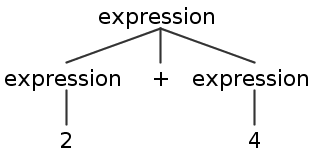
\includegraphics[scale=0.4]{pics/antlr4_parse_tree_visitAdditionVisitNumberBeispiel.png}
\caption{Syntaxbaum für beispielhaften arithmetischen Ausdruck}
\end{figure}
\pagebreak
Zunächst wird die visitAddition-Methode aufgerufen, da der Operator der expression das ''+'' Zeichen ist. Die visitChildren-Methode gibt nun die Zeichenkette
\begin{lstlisting} [frame=single]
ldc 2
ldc 4
\end{lstlisting}
zurück, da die untergeordneten Expressions nur Zahlen enthalten. Dem fügt die visitAddition-Methode wiederrum den Befehl
\begin{lstlisting} [frame=single]
iadd
\end{lstlisting}
hinzu, um die Addition durchzuführen.
\linebreak

In der JavaVM werden diese Instruktionen wie folgt verarbeitet:
Im Initialzustand ist der Stack leer.

\begin{figure}[h!]
\centering
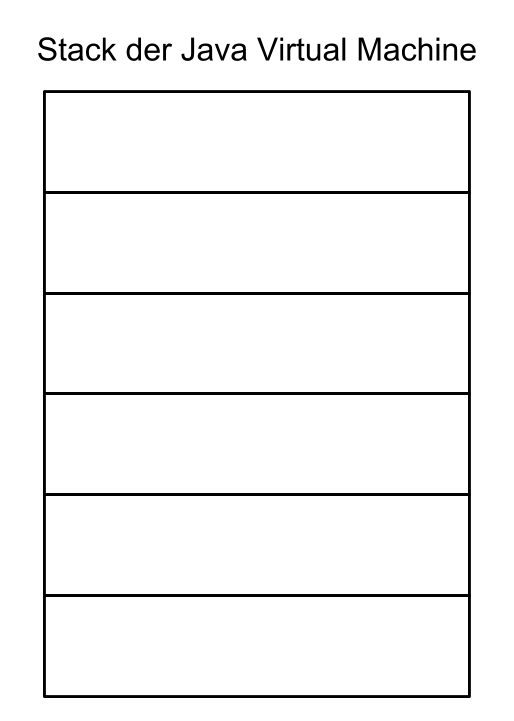
\includegraphics[scale=0.2]{pics/stack_visual.png}
\caption{Zustand des Kellerspeicher der JavaVM}
\end{figure}

Der Befehl \textit{ldc 2} legt den Wert \textit{2} auf den Stack.

\begin{figure}[h!]
\centering
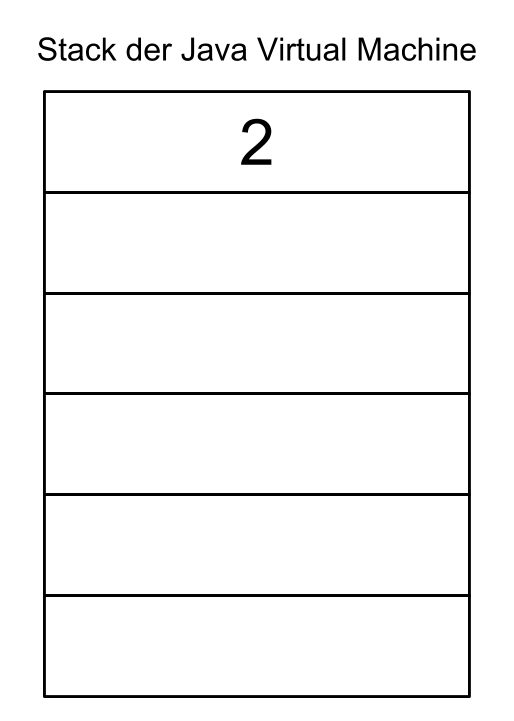
\includegraphics[scale=0.2]{pics/stack_visual(1).png}
\caption{Zustand des Kellerspeicher der JavaVM}
\end{figure}

Der Befehl \textit{ldc 4} legt den Wert \textit{4} auf den Stack.

\begin{figure}[h!]
\centering
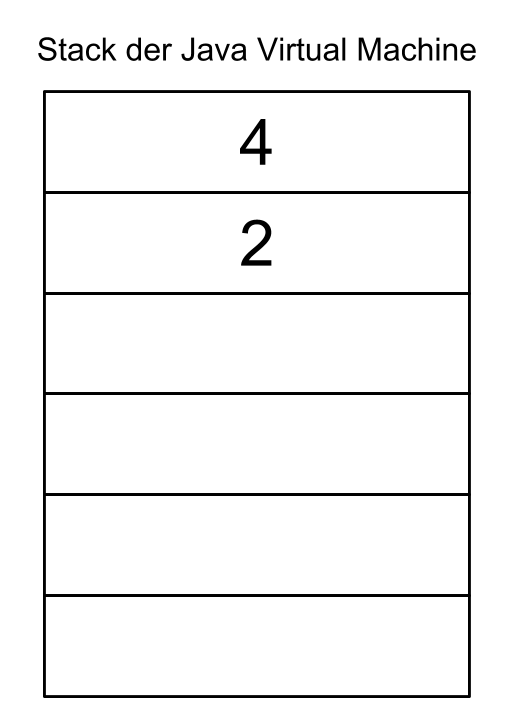
\includegraphics[scale=0.2]{pics/stack_visual(2).png}
\caption{Zustand des Kellerspeicher der JavaVM}
\end{figure}

Der Befehl \textit{iadd} nimmt zwei Werte vom Stack und legt das Ergebnis der Addition dieser Werte wieder auf den Stack

\begin{figure}[h!]
\centering
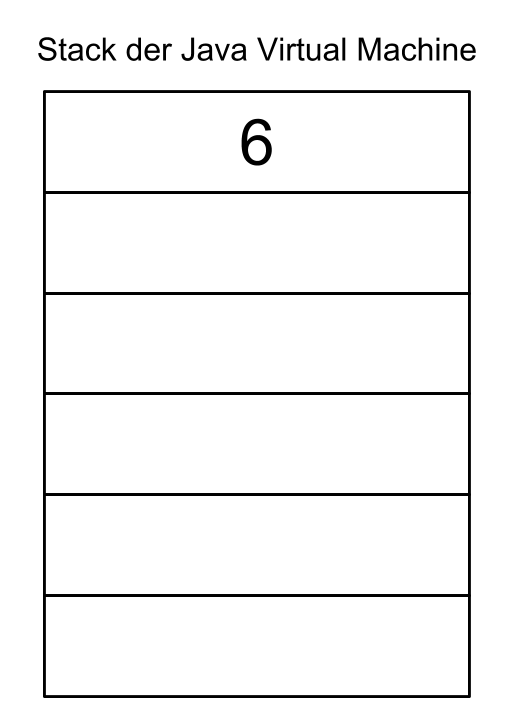
\includegraphics[scale=0.2]{pics/stack_visual(3).png}
\caption{Zustand des Kellerspeicher der JavaVM}
\label{fig:method}
\end{figure}



\pagebreak

\subsection{Ausweiten der simplen Grammatik}
Nachdem die Sprache grundlegende Funktionalität erhielt, versuchten wir die weiteren Bestandteile, die durch die Anforderungen festgelegt wurden, zu implementieren. 


\subsubsection{Ergebnisausgabe}
Ein Programm ohne Ausgabe ergibt keinen Sinn, da das berechnete Ergebnis nicht betrachtet werden kann. Eine Ausgabefunktion zu implementieren stellte sich hier nicht als zu großes Problem heraus, da Jasmin die Fähigkeit besitzt Objekte und Methoden der Java Library zu nutzen. Wir nutzen dies und implementierten die Ausgabefunktion wie folgt:

\scriptsize \begin{lstlisting}[frame=single]
/**@brief
 * vearbeitet den Aufruf der println-Funktion
 */
public String visitPrintln(PrintlnContext ctx) {
	return  ";calling println\n" + 
		//legt ein System.out Objekt auf den Stack
		"getstatic java/lang/System/out Ljava/io/PrintStream;\n" + 	
		//Argument der print-Funktion
		visit(ctx.argument) + 						
		//ruft die Methode println des System.out-Objekts auf
		"invokevirtual java/io/PrintStream/println(I)V\n\n"; 				
}
\end{lstlisting}

\normalsize
Es wird zuerst ein System.out-Objekt auf den Stack gelegt, danach der auszugebende Wert. Schließlich folgt der Aufruf der Methode println(), die das Argument sowie das System.out-Objekt vom Stack wieder herunternimmt.


Der Aufruf in unserer Programmiersprache lautet: 
\begin{lstlisting}[frame=single]
println( argument );
\end{lstlisting}

\subsection{Implementierung von Variablen}
Eine Variable wird folgendermaßen deklariert:
\begin{lstlisting}[frame=single]
int NAME;
\end{lstlisting}
Stößt der Compiler im Parsetree auf solch eine Zeile, wird geprüft, ob bereits eine Variable mit dem selben Namen im Programm existiert. Ist dies der Fall, wird eine Exception geworfen und der Kompiliervorgang bricht ab. Existiert der Name der Variablen noch nicht im Programm wird ein neuer Eintrag in der Variablentabelle erstellt.

Um einer deklarierten Variable einen Wert zuzuweisen, wird folgende Syntax verwendet:
\begin{lstlisting}[frame=single]
NAME = EXPRESSION;
\end{lstlisting}
Wobei die EXPRESSION sich zu einem Wert evaluieren lassen muss.
Wird eine solche Anweisung erkannt, wird zuerst versucht, den Namen der Variablen zu dem dazugehörigen Index der Variablentabelle auszuwerten. Gelingt dies nicht, wurde die Variable nicht deklariert und es wird eine Exception geworfen. Kann der Name der Variablen zu einem Index ausgewertet werden, wird die Variable mit 
\begin{lstlisting}[frame=single]
visit(ctx.expr)
\end{lstlisting}
auf den Stack gelegt und mit ''istore [index]'' der Wert der Variablen in der Jasmin-Variablentabelle gespeichert.

Eine Variable wird über ihren Namen als Teil einer Expression aufgerufen. Hier wird dann intern der Name zum Index der Variable aufgelöst. Gelingt dies nicht, wurde die Variable nicht deklariert und es wird eine Exception geworden. Ansonsten wird mit
''iload [index]'' der Wert der Variablen zur Verarbeitung auf den Stack der JavaVM gelegt.

\subsection{Implementierung von Funktionen}
Bevor der eigentliche Visitor arbeitet, wird der gesamte Baum auf Funktionsdeklarationen untersucht. Dies sorgt dafür, dass Funktionen an beliebigen Stellen im Quellcode definiert werden können und keine Vorwärtsdeklarationen notwendig sind. Die gefundenen Funktionen werden in einer Liste gespeichert.

Funktionen werden mit folgender Syntax deklariert:
% ToDo: Bitte einfügen

Stößt der Compiler auf solch eine Syntax, wird anhand einer Funktionsliste geprüft, ob eine Funktion mit einer solchen Signatur bereits existiert. Ist dies so, wird eine Exception geworfen und der Kompiliervorgang bricht ab. Andernfalls wird ein neuer Eintrag mit dem Namen und der Signatur der Funktion in die Funktionsliste eingefügt.

Beim Aufruf von Funktionen wird ebenfalls geprüft, ob eine Funktion mit der gegebenen Signatur existiert. Existiert die Funktion nicht, wird eine Exception geworfen, andernfalls wird die vorher verwendete Variablentabelle gesichert und eine neue Variablentabelle für die Funktion angelegt. Dies ermöglicht die Realisierung von Variablen-Scopes. Danach werden die Argumente und Instruktionen der Funktion durch
\begin{lstlisting}[frame=single]
invokestatic [functionname] ([ggf. parameter])
\end{lstlisting}
bearbeitet.
Nach dem Abarbeiten der Funktion wird die vorherige, gesicherte Variablentabelle wieder hergestellt.

\subsection{Implementierung von Konstanten}
Konstanten sind intern als Erweiterung von Variablen anzusehen. 
Zusätzlich zu Variablen werden bei konstanten folgende Schritte ausgeführt:
Wird eine Konstante deklariert, wird deren hasBeenAssigned-Flag auf false gesetzt.
Bei der Wertzuweisung zu der Konstanten wird geprüft, welchen Wert dieses Flag besitzt. Ist der Wert false, wird eine normale Zuweisung durchgeführt und der Wert des Flags auf true gesetzt. Ist der Wert true, wurde der Konstanten bereits eine Wert zugewiesen und eine weitere Zuweisung kann nicht erfolgen. Es wird eine Exception geworfen und der Kompiliervorgang bricht ab.

\subsection{Implementierung von Bedingten Verzweigungen}
Verzweigungen sind in drei Teile aufzuteilen:
\begin{itemize}
	\item conditionInstructions
	\item onTrueInstructions
	\item onFalseInstructions	
\end{itemize}

Wird auf eine conditionInstruction getroffen, wird diese bearbeitet.
Evaluiert die Expression zu true, werden die onTrueInstructions ausgeführt, die onFalseInstructions werden übersprungen. Evaluiert die conditionInstruction zu false, werden die onTrueInstructions übersprungen und die onFalseInstructions ausgeführt.
Um die entsprechenden Instruktionen zu überspringen, werden Labels benötigt, die markieren, an welche Stelle des Programms gesprungen werden kann. Damit die Labels für jede Verzweigung einzigartig sind, wird gezählt, wie oft Verzweigungen vorkommen und die Labels werden entsprechend benannt.

Evaluiert werden die Bedingungen wie folgt:
Ergibt die Expression 0, gilt sie als false, alle anderen Werte gelten als true.
Erlaubte Operatoren der conditionInstruction-Expression sind folgende Operatoren:
\begin{itemize}
	\item Vergleiche (<, <=, >, >=, ==)
	\item Logik-Gatter (\& \&, ||, !)
\end{itemize}

\subsection{Implementierung einer Schleife}
Eine Schleife kann intern aufgeteilt werden in
\begin{itemize}
\item Bedingung
\item Befehle, auszuführen, wenn Bedingung wahr ist
\end{itemize}

Im Pseudocode sieht eine Schleife folgendermaßen aus:
\\
\begin{algorithm}[H]
	conditionLabel \\
	conditionInstructions \\
		\If{conditionInstructions == true}
		{ 
			Sprung zu onTrueLabel
		}
		\If{conditionInstruction == false}
		{
			Sprung zu endOfWhileLabel
		}
	[onTrueLabel] \\
	onTrueInstructions \\
	Sprung zu conditionLabel \\	
	endOfWhileLabel
\end{algorithm}
\(\)\\
Die Labels werden benötigt, damit in der Schleife an die entsprechende Stelle gesprungen werden kann. Damit intern die Labels zur richtigen Schleife zugeordnet werden können, wird mitgezählt, wie oft Schleifen im Programm verwendet werden.

\subsection{Dokumentation}
Zur effizienten Erstellung der Dokumentation wurde \LaTeX \(\) in Verbindung mit TexMaker verwendet. Dazu wurden die einzelnen Hauptüberschriften in eigene Dateien ausgelagert und in der Hauptdatei inkludiert. Dies hat eine erhöhte Übersichtlichkeit zur Folge.
Um die Dokumentation versioniert zu speichern, wurde diese im verwendeten Git-Repository hochgeladen. Damit keine unnötigen Entwicklungs- bzw. Zwischenschrittdateien von \LaTeX \(\) in das verwendete Git-Repository übernommen werden, wurde ein Alias erstellt, der ebendiese Dateien beim Alias-Aufruf automatisiert entfernt. Dieser Alias sieht wie folgt aus:

\begin{lstlisting}[frame=single]
rmtex_dev()
{
	echo "Removing .aux"
	rm *.aux &> /dev/null
	echo "Removing .toc"
	rm *.toc &> /dev/null
	echo "Removing .synctex.gz"
	rm *.synctex.gz &> /dev/null
	echo "Removing .log"
	em *.log &> /dev/null
	echo "Removing .out"
	rm *.out &> /dev/null
}
\end{lstlisting}